\documentclass{beamer}
\usepackage{multicol,lipsum,caption,graphicx}
\usepackage{mathtools, amsmath,booktabs,verbatim,tikz} 
\usetikzlibrary{shapes.geometric, arrows,positioning,matrix,calc}
\usepackage{booktabs, makecell, amsmath,afterpage}
\usepackage{tikz,tabularx, adjustbox}
%\usepackage{mathptmx}

\newcommand\scalemath[2]{\scalebox{#1}{\mbox{\ensuremath{\displaystyle #2}}}}

\usetheme[progressbar=frametitle]{metropolis}
\setbeamertemplate{frame numbering}[fraction]
\useoutertheme{metropolis}
\useinnertheme{metropolis}
\usefonttheme{metropolis}
\usecolortheme{spruce}
\setbeamercolor{background canvas}{bg=white}

\title{Paper Progress Report}
\author{Huiyao Zhang}
\institute{Kyoto Institue of Technology}
\date{03-23-2021}
\setbeamertemplate{itemize/enumerate body begin}{\large}

\DeclarePairedDelimiter\Floor\lfloor\rfloor
\DeclarePairedDelimiter\Ceil\lceil\rceil
\begin{document}
\begin{frame}
    \titlepage
\end{frame}

\begin{frame}[c]{Content} 
    \begin{enumerate}
        \item Optimum design of laminated composites for minimum thickness by a variant of genetic algorithm
        \item A technique for constrained optimization of cross ply laminates useing a new variant of genetic algorithm
        \item An approximation method of classic lamination theory based on evolutionary artificial neural network.
    \end{enumerate}
\end{frame}

\begin{frame}[c]{Content} 
    \begin{enumerate}
        \item Classic lamination theory
        \item Failure theory for composite material
        \item Self-adaptative genetic algorithm
        \item Experiment and result
        \item Comparison with related research
    \end{enumerate}
\end{frame}



\begin{frame}{1. Classic Lamination Theory}
    \begin{columns}[c]
    \begin{column}{0.5\textwidth}
		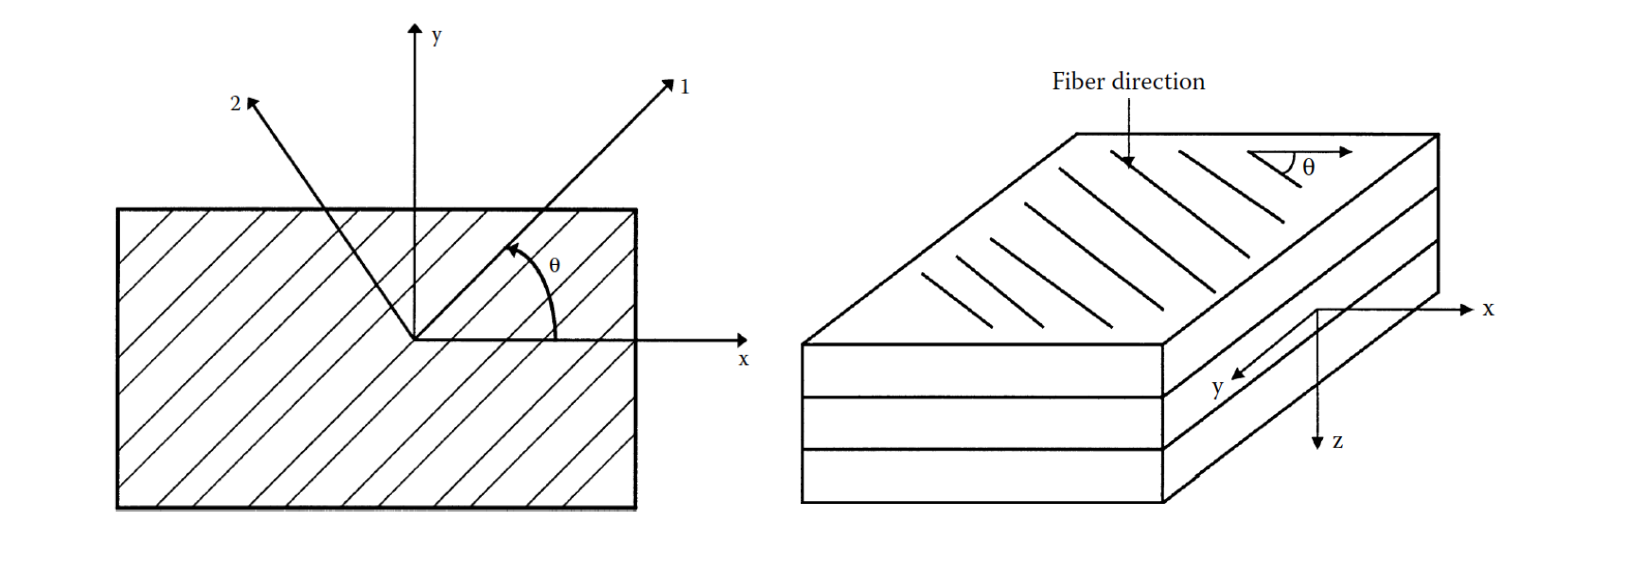
\includegraphics[width=1.5\linewidth]{./fig/lamina_local_global_axes.png}
        \captionof{figure}{Composite Material}
    \end{column}
	\begin{column}{0.5\textwidth}
		\begin{equation} \label{eq:force_and_moments}
			\begin{array}{l}
				\begin{aligned}
			\begin{bmatrix}
				N_x \\
				N_y \\
				N_{xy}
			\end{bmatrix}
			&=
			\begin{bmatrix}
				A_{11} & A_{12} & A_{16} \\
				A_{12} & A_{22} & A_{26} \\
				A_{16} & A_{26} & A_{66} 
			\end{bmatrix}
			\begin{bmatrix}
				\varepsilon_x^0 \\
				\varepsilon_y^0 \\
				\gamma_{xy}^0
			\end{bmatrix}   \\
			&+               
			\begin{bmatrix}
				B_{11} & B_{12} & B_{16} \\
				B_{11} & B_{12} & B_{16} \\
				B_{16} & B_{26} & B_{66} 
			\end{bmatrix}
			\begin{bmatrix}
				k_x \\
				k_y \\
				k_{xy} 
			\end{bmatrix}  \\
		\end{aligned} \\ \\
		\begin{aligned}
			\begin{bmatrix}
				M_x \\
				M_y \\
				M_{xy}
			\end{bmatrix}
			&=
			\begin{bmatrix}
				B_{11} & B_{12} & B_{16} \\
				B_{12} & B_{22} & B_{26} \\
				B_{16} & B_{26} & B_{66} 
			\end{bmatrix}
			\begin{bmatrix}
				\varepsilon_x^0 \\
				\varepsilon_y^0 \\
				\gamma_{xy}^0
			\end{bmatrix} \\ 
			&+  
			\begin{bmatrix}
				D_{11} & D_{12} & D_{16} \\
				D_{11} & D_{12} & D_{16} \\
				D_{16} & D_{26} & D_{66} 
			\end{bmatrix}
			\begin{bmatrix}
				k_x \\
				k_y \\
				k_{xy} 
			\end{bmatrix}
		\end{aligned}
			\end{array}
		\end{equation}
	\end{column}
\end{columns}
\end{frame}

\begin{frame}{2. Failure Theory }
\begin{columns}[c]
    \begin{column}{0.4\textwidth}
		\begin{figure}
		\centering
		\resizebox{1.2\linewidth}{!}{
		\begin{tikzpicture}
			\begin{scope}
				%\draw[style=help lines] (-3,-3) grid (3,3);
				\draw (0,0) rectangle (2,3);
				\draw[->] (1.3,1.2) -- (2.6,1.2);
				\draw[->] (1.3,1.2) -- (1.3,3.4);
				\node at (2.2,1) {$X_T$};
				\node at (1.5, 3.2) {$Y_T$};
				\node at (-0.2, 0.9) {$X_C$};
				\node at (1.8, -0.2) {$Y_C$};
			\end{scope}
			\begin{scope}[xshift=6cm,yshift=1.15cm]
				%\draw[style=help lines] (-3,-3) grid (3,3);
				\draw[rotate=30] (0,0) ellipse (2cm and 1cm);
				\draw[->] (0.2,0) -- (0.2,2.2);
				\draw[->] (0.2,0) -- (1.9,0);
				\node at (1.6,-0.2) {$X_T$};
				\node at (0.3, 1.3) {$Y_T$};
				\node at (-1.6, 0) {$X_C$};
				\node at (-0.5, -1.5) {$Y_C$};
			\end{scope}
		\end{tikzpicture}
		}
		\caption{Schematic failure surfaces for maximum stress and quadratic failure
		criteria}
		\end{figure}
    \end{column}
    \begin{column}{0.6\textwidth}
		\begin{itemize}
			\item  Maximum stress failure
				\begingroup
				\small
				\begin{align*}
					SF_{MS}^k = \text{min of}
					\begin{cases}
						SF_X^k = 
						\begin{cases}
							\frac{X_t}{\sigma_{11}}, \text{ if } \sigma_{11}>0 \\
							\frac{X_c}{\sigma_{11}}, \text{ if } \sigma_{11}<0 \\
						\end{cases} \\
						SF_Y^k = 
						\begin{cases}
							\frac{Y_t}{\sigma_{22}}, \text{ if } \sigma_{22}>0 \\
							\frac{Y_c}{\sigma_{22}}, \text{ if } \sigma_{22}<0 \\
						\end{cases} \\
						SF_S^k =
						\begin{cases}
							\frac{S}{|\tau_{12}|} \\
						\end{cases} \\
					\end{cases} \textstyle{.}
				\end{align*}
				\endgroup
			\item  Tsai-wu failure theory

		 \begingroup
		 \small
		 \begin{equation*} 
		 \begin{split}
			H_1 \sigma_1  & + H_2 \sigma_2 + H_6 \tau_{12} + H_{11}\sigma_1^2 + H_{22} \sigma_2^2 \\
						  & + H_{66}  \tau_{12}^2 + 2H_{12}\sigma_1\sigma_2 < 1
		 \end{split}
		\end{equation*}
		\endgroup
		\end{itemize}
    \end{column}
\end{columns}
\end{frame}

\begin{frame}{2. Traditional GA model}
	\begin{figure}
\centering
	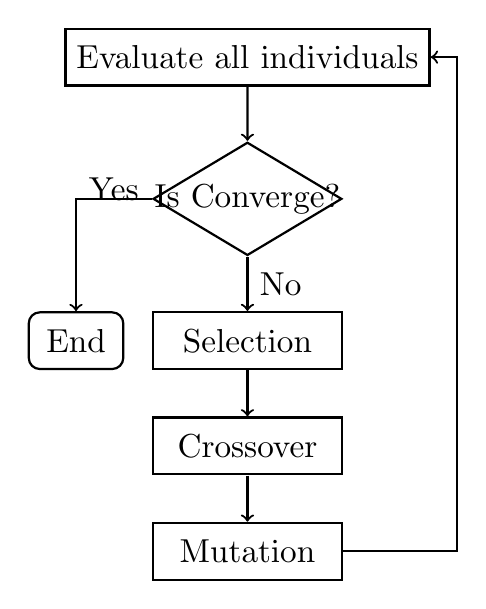
\begin{tikzpicture}[thick, scale=1.2, every node/.style={transform shape}]
		\tikzstyle{startstop} = [rectangle, rounded corners, minimum width=1.0cm,minimum height=0.6cm, text centered, draw=black]
		\tikzstyle{io} = [trapezium, trapezium left angle=70, trapezium right angle=110, minimum width=2cm, minimum height=0.6cm, text centered, draw=black]
		\tikzstyle{process} = [rectangle, minimum width=2cm, minimum height=0.6cm, text centered, draw=black]
		\tikzstyle{decision} = [diamond,minimum width=2cm, minimum height=1.2cm, draw=black]
		\node (fitness) [process] {Evaluate all individuals};
		\node[yshift=-0.5cm] (decision) [decision, below of=fitness] {} node at (decision.base) {Is Converge?};
		\node[yshift=-0.5cm] (selection) [process, below of=decision] {Selection};
		\node (crossover) [process] at ($(selection.south)+(0,-0.8cm)$) {Crossover};
		\node (mutation) [process] at ($(crossover.south)+(0,-0.8cm)$)  {Mutation};
		\node (end) [startstop] at ($(selection.west)+(-0.8cm,0cm)$) {End};

		\draw [->] (fitness) -- (decision);
		\draw [->] (decision.south) -- (selection.north) node[auto=left,pos=0.5]{No};
		\node at ($(decision.west)+(-0.4cm, 0.1cm)$) {Yes};
		\draw [->] (selection.south) -- (crossover.north);
		\draw [->] (crossover.south) -- (mutation.north);
		\draw [->] (decision.west) -| (end.north);
		\draw [->] (mutation.east) -- ($(mutation.east)+(1.2cm,0cm)$) |-
			(fitness.east);
	\end{tikzpicture}
\caption{Traditional GA Model.}
\label{fig:old_ga_model}
\end{figure}

\end{frame}

\begin{frame}{3. New GA model}
	
\begin{figure}
\begin{center}
	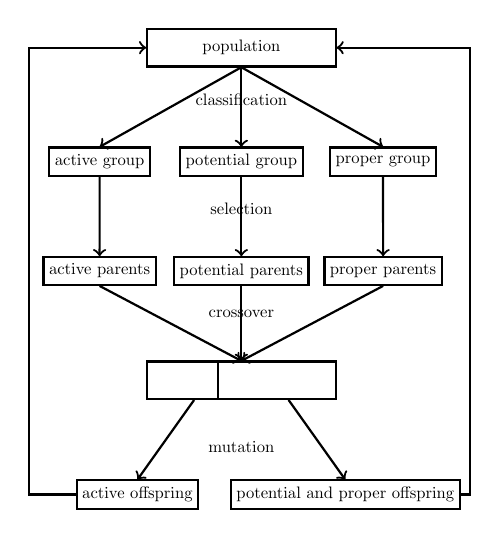
\begin{tikzpicture}[thick, scale=0.6, every node/.style={transform shape}]
	\tikzstyle{rec} = [rectangle, minimum width=4cm, minimum height=0.8cm,
	text centered, draw=black]
	\tikzstyle{subgroup} = [rectangle, minimum width=1.5cm, minimum height=0.6cm,
	text centered, draw=black]
	\tikzstyle{bigsubgroup} = [rectangle, minimum width=2.5cm, minimum height=0.6cm,
	text centered, draw=black]
	% population
	\node (population) [rec] {population};
	% active group
	\node (active_group_1) at ($(population.south)+(-3cm, -2.0cm)$) [subgroup]
		{active group};
	\node (active_group_2) at ($(active_group_1.south)+(0cm, -2.0cm)$)
		[subgroup] {active parents};
	\draw[->] (population.south) -- (active_group_1.north);
	\draw[->] (active_group_1.south) -- (active_group_2.north);
	% potential group
	\node (potential_group_1) at ($(population.south)+(0cm, -2.0cm)$) [subgroup]
		{potential group};
	\node (potential_group_2) at ($(potential_group_1.south)+(0cm, -2.0cm)$)
		[subgroup] {potential parents};
	\draw[->] (population.south) -- (potential_group_1.north);
	\draw[->] (potential_group_1.south) -- (potential_group_2.north);
	\node at ($(potential_group_1.north)+(0cm, 1.0cm)$) {classification };
	\node at ($(potential_group_2.north)+(0cm, 1.0cm)$) {selection};
    % proper group
	\node (proper_group_1) at ($(population.south)+(3cm, -2.0cm)$) [subgroup]
		{proper group};
	\node (proper_group_2) at ($(proper_group_1.south)+(0cm, -2.0cm)$)[subgroup]
		{proper parents};
	\draw[->] (population.south) -- (proper_group_1.north);
	\draw[->] (proper_group_1.south) -- (proper_group_2.north);
	% crossover
	\node (after_cross_over) at ($(potential_group_2.south)+(0cm, -2.0cm)$) [rec] {};
	\node  at ($(after_cross_over.north)+(0cm, 1.0cm)$)  {crossover};
	\draw[-] ($(after_cross_over.south)+(-0.5cm,0cm)$) --
		($(after_cross_over.north)+(-0.5cm,0cm)$);
	\draw[->] (active_group_2.south) -- (after_cross_over.north);
	\draw[->] (potential_group_2.south) -- (after_cross_over.north);
	\draw[->] (proper_group_2.south) -- (after_cross_over.north);
	% mutation
	\node (active_group_3) at ($(after_cross_over.south)+(-2.2cm, -2.0cm)$)
		[subgroup] {active offspring};
	\node at ($(after_cross_over.south)+(0cm, -1.0cm)$) {mutation};
	\draw[->] ($(after_cross_over.south)+(-1cm,0cm)$)--(active_group_3.north);
	\node (poteni_and_prop) at ($(after_cross_over.south)+(2.2cm, -2.0cm)$)
		[bigsubgroup] {potential and proper offspring};
	\draw[->] ($(after_cross_over.south)+(1cm,0cm)$)--(poteni_and_prop.north);

	% final draw
	\draw[->] (poteni_and_prop.east) --($(poteni_and_prop.east) + (0.2cm,0cm)$) |- (population.east);
	\draw[->] (active_group_3.west) -- ($(active_group_3.west) + (-1cm,0cm)$)
		|- (population.west);
\end{tikzpicture}
\end{center}
\caption{GA Model\label{GA:model}}
\end{figure}

\end{frame}

\begin{frame}{3. New GA: selection operator}
    \begin{columns}[c]
    \begin{column}{0.5\textwidth}
		\begin{itemize}
			\item acitve group: individual is used to increase the diversity of the population
			\item potential group: individual doesn't fulfill constraint
			\item proper group: individual meet constraint
		\end{itemize}
    \end{column}
	\begin{column}{0.5\textwidth}
		\begin{figure}
			\caption{Parents}
			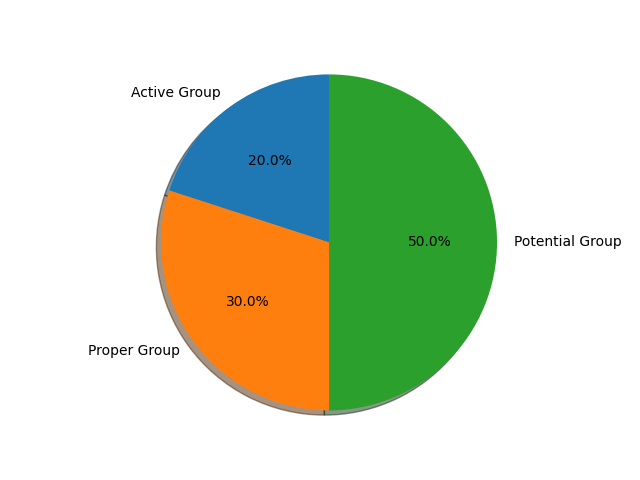
\includegraphics[scale=0.5]{fig/chapter2_figure_group_pie.png}
		\end{figure}
	\end{column}
\end{columns}
\end{frame}

\begin{frame}{3. Self-adaptative GA}
    \begin{columns}[c]
    \begin{column}{1\textwidth}
		\begin{itemize}
			\item Modifying selection strategy: in order to handle the constraint search
			\item Self-adaptative mutation direction of fiber orientation and laminate thickness:
				random change the length, and the angle in the laminate.
			\item The self-adaptative parameters don't refer to parent's proportion, mutation
				probability.
		\end{itemize}
    \end{column}
    \begin{column}{0.8\textwidth}

    \end{column}
\end{columns}
\end{frame}


\begin{frame}{3. Self-adaptative GA:  mutation operator}
    \begin{columns}[c]
    \begin{column}{1\textwidth}
		$\text{md} = [CT_1, \cdots, CT_{n-1}, CT_n] -  [ICV_0, \cdots, ICV_{n-1},
		ICV_n]$ \\
		\begin{itemize}
			\item  md means mutation direction.
			\item  $CT_i$ denotes the i-th constraint, such as weight, safety factor.
			\item  $ICV_i$ denotes individual's i-th constraint value, such as,  weight, safety
				factor of current individual.
		\end{itemize}

    \end{column}
\end{columns}
\end{frame}


\begin{frame}{4. Self-adaptative GA:  mutation operator}
    \begin{columns}[c]
	\begin{column}{1\textwidth}
		\begin{itemize}
			\item length mutation =  
				\[
				  \begin{cases}
					  LMC*[0, \sum_{i=1}^{N}{md_i}] & \text{if $\sum_{i=1}^{N}{md_i} > 0$} \\
					  LMC*[\sum_{i=1}^{N}{md_i}, 0] & \text{if $\sum_{i=1}^{N}{md_i} < 0$} \\
				  \end{cases}
				\] \\
				LMC stands for length mutation coefficient, it's a positive integer.
			\item angle mutation = 
				\[
				  \begin{cases}
					  AMC*[0, \sum_{i=1}^{N}{md_i}] & \text{if $\sum_{i=1}^{N}{md_i} > 0$} \\
					  AMC*[\sum_{i=1}^{N}{md_i}, 0] & \text{if $\sum_{i=1}^{N}{md_i} < 0$} \\
				  \end{cases}
				\] \\
				AMC stands for angle mutation coefficient, it's sign is unclear.
		\end{itemize}
	\end{column}
\end{columns}
\end{frame}

\begin{frame}{Paper 1: Cross ply laminate}
	\begin{figure} 
	\centering
	\caption{Model for cross ply laminate}
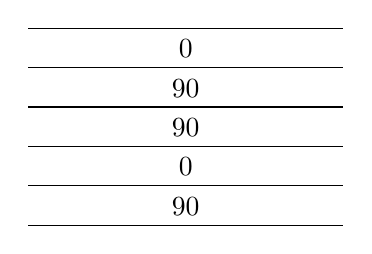
\begin{tikzpicture}
	\draw (0,0) -- (4,0);
	\draw (0,-0.5) -- (4,-0.5) node[midway, above] {$0$};
	\draw (0,-1) -- (4,-1) node[midway, above] {$90$} ;
	\draw (0,-1.5) -- (4,-1.5) node[midway, above] {$90$};
	\draw (0,-2) -- (4,-2) node[midway, above] {$0$};
	\draw (0,-2.5) -- (4,-2.5) node[midway, above] {$90$};
\end{tikzpicture}
\end{figure}

\end{frame}

\begin{frame}{Paper 1: Experiment}
    \begin{columns}[c]
    \begin{column}{0.5\textwidth}
		\begin{figure}
			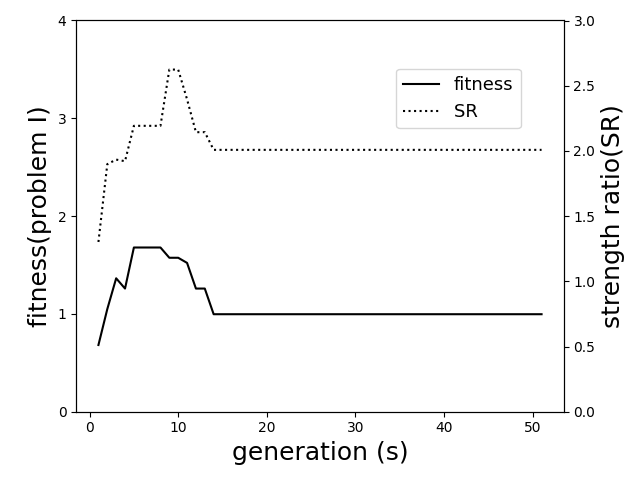
\includegraphics[scale=0.4]{fig/chapter4_first_result_strength_ratio_and_fitness.png}
			\caption{Parents}
		\end{figure}
    \end{column}
	\begin{column}{0.5\textwidth}
		\begin{figure}
			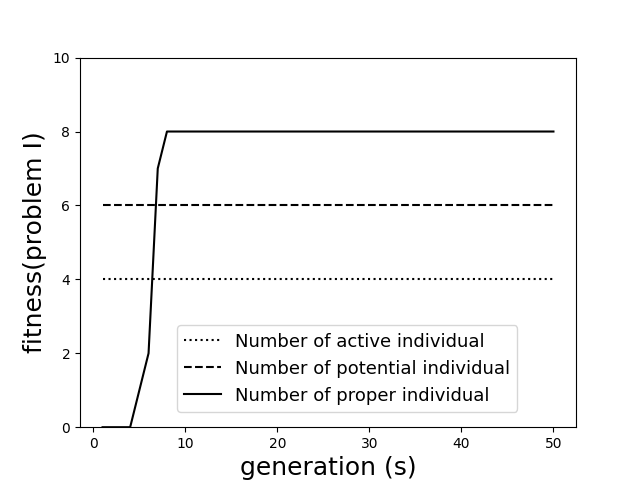
\includegraphics[scale=0.4]{fig/chapter4_first_result_number_of_three_groups.png}
			\caption{Parents}
		\end{figure}
	\end{column}
\end{columns}
\end{frame}

\begin{frame}{Paper 1: Comparison}
	\begin{table*}[!htb]
\caption{The optimum lay-ups for the loading $N_x=1e6$ N}
\centering
\begin{adjustbox}{width=1\textwidth}
\begin{tabular}{c|cc|cc}
	\toprule
	Cross Ply $[0_M/90_N]$         & \multicolumn{2}{c}{Previous Research} & \multicolumn{2}{c}{Current Research} \\
	\midrule																								  
	 Material       &  Glass-Epoxy & Graphite-Epoxy  & Glass-Epoxy & Graphite-Epoxy      \\ 
	      M         &  68          &    17           &  78		    &  18             \\
	      N         &  72          &    18           &  28		    &  8              \\
no. of lamina(n)    &  140         &    35           &  106	    &  26                     \\
         SR         &  2.01        &    2.10         &  2.03	    &  2.16            \\
     weight         &  9.10        &    1.84         &  6.89	    &  102.5           \\
	\bottomrule
\end{tabular}
\end{adjustbox}
\label{tab:comparsion}
\end{table*}

\end{frame}



\begin{frame}{Paper 2: Loading $N_x = 10, N_y=5 $ MPa m}
    \begin{columns}
    \begin{column}{0.5\textwidth}

        \begin{center}
			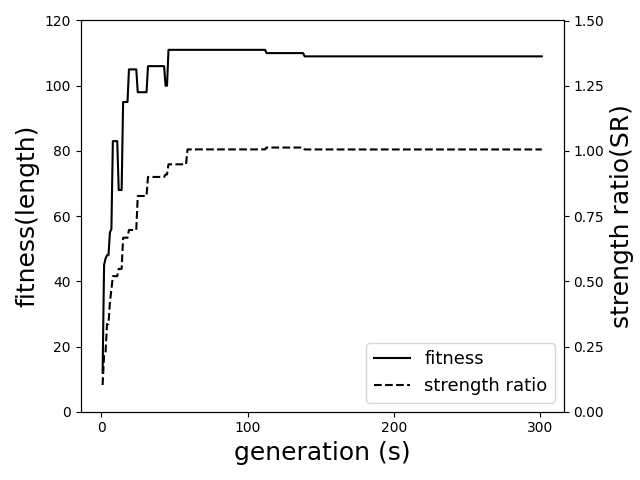
\includegraphics[width=1.0\linewidth]{./fig/two_distinct_angle_fitness_and_sr.png}
        \end{center}

        \begin{center}
			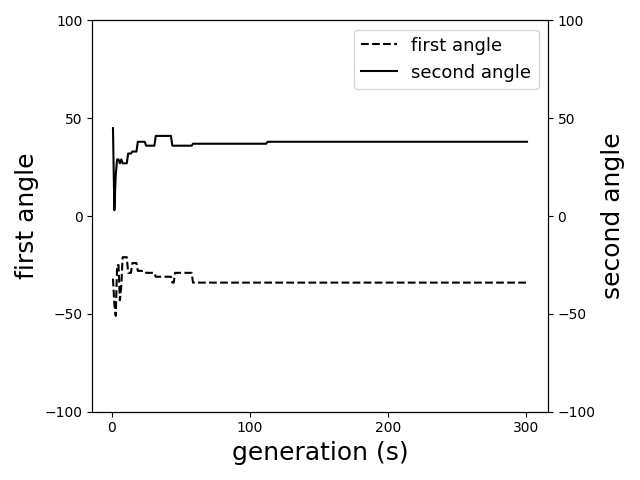
\includegraphics[width=1.0\linewidth]{./fig/two_distinct_angle_angle_change.png}
        \end{center}
    \end{column}
    \begin{column}{0.5\textwidth}
        \begin{center}
			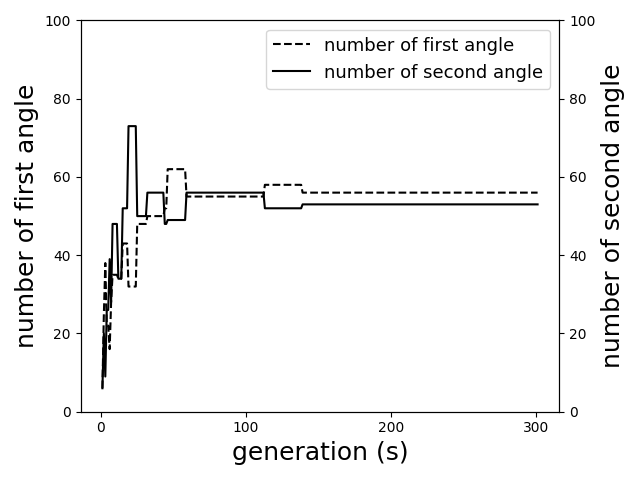
\includegraphics[width=1.0\linewidth]{./fig/two_distinct_angler_number_change.png}
              \captionof{figure}{Two distinct angles in the laminate}
        \end{center}
    \end{column}
\end{columns}
\end{frame}


\begin{frame}{Paper 2: Comparison}
\begin{table}
	\normalsize
	\caption{Comparison with the results of DSA}
	\label{tab:comparision}
	\centering
	\resizebox{10cm}{!}{
\begin{tabular}{c|cccc|lccc}
	\toprule
	\textbf{Loading}	    & \multicolumn {4}{c}{\textbf{Akbulut and Sonmez's Study}}   & \multicolumn {4}{c}{\textbf{Present Study}}\\
	\midrule
	 $N_{x}/N_{y}/N_{xy}$   & Optimum lay-up			        & laminate  & TW & MS   & Optimum lay-up & laminate  & TW & MS \\
	  (MPa m)	            & sequences					        & thickness &    &      & sequences	     & thickness &    &    \\
	\midrule
	  10/5/0                 &  $[37_{27}/\text{-}37_{27}]_s$     &  108      &  1.0068  &  1.0277 & $[33_{29}/\text{-}39_{25}/\bar{\text{-}39}]_s$     &     109      &  1.0074      &  1.0246  \\
	  20/5/0                 &  $[31_{23}/\text{-}31_{23}]_s$     &  92       &  1.0208  &  1.1985 & $[33_{22}/\text{-}31_{24}]_s$                      &     92      &  1.0055       &  1.2065    \\
	  40/5/0                 &  $[26_{20}/\text{-}26_{20}]_s$     &  80       &  1.0190  &  1.5381 & $[29_{18}/\text{-}21_{23}/\bar{\text{-}21}]_s$     &     83      &  1.0034       &  1.7350   \\
	  80/5/0                 &  $[21_{25}/\text{-}19_{28}]_s$     &  106      &  1.0113  &  1.2213 & $[\text{-}20_{27}/21_{25}/\bar{25}]_s$             &     105      &  1.0029      &  1.2063    \\
	  120/5/0                &  $[17_{35}/\text{-}17_{35}]_s$     &  140      &  1.0030  &  1.0950 & $[\text{-}18_{34}/17_{36}]_s$                     &     140      &  1.0000      &  1.0898     \\
	\bottomrule
\end{tabular}
}
\end{table}
\end{frame}

\begin{frame}{Paper 3: }
	\begin{figure}
\centering
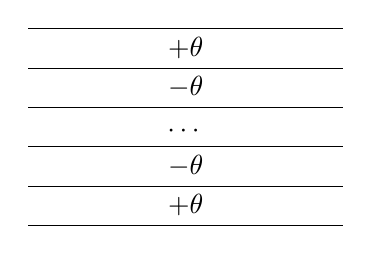
\begin{tikzpicture}
	\draw (0,0) -- (4,0);
	\draw (0,-0.5) -- (4,-0.5) node[midway, above] {$\mathit{+}\theta$};
	\draw (0,-1) -- (4,-1) node[midway, above] {$\mathit{-}\theta$} ;
	\draw (0,-1.5) -- (4,-1.5) node[midway, above] {$\cdots$};
	\draw (0,-2) -- (4,-2) node[midway, above] {$\mathit{-}\theta$};
	\draw (0,-2.5) -- (4,-2.5) node[midway, above] {$\mathit{+}\theta$};
\end{tikzpicture}
\caption{Model for Angle ply laminate}
\end{figure}


\end{frame}

\begin{frame}{Paper 3: }
	
\begin{figure}
	\begin{center}
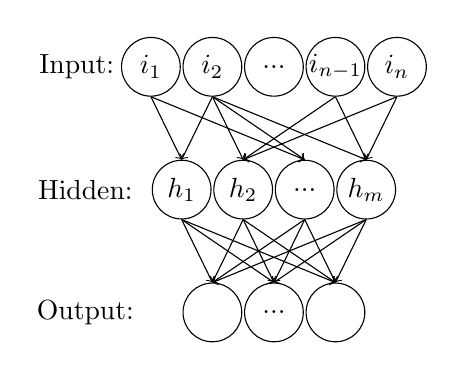
\begin{tikzpicture}
[ plain/.style={ draw=none, fill=none, }, remember picture, net/.style={ matrix of nodes, nodes={ draw, circle,
    inner sep=7.5pt
    },
  nodes in empty cells,
  column sep=-10.5pt,
  row sep=0.8cm
  }
]
%\draw[help lines] (-3cm,-6cm) grid (6cm,3cm);
\matrix[net] (mat)
{
              & |[plain]| &           & |[plain]|  &           & |[plain]| &           &  |[plain]|      &               \\
    |[plain]| &           & |[plain]| &            & |[plain]| &           & |[plain]| &                 & |[plain]|     \\ 
    |[plain]| & |[plain]| &           & |[plain]|  &           & |[plain]| & 	  	   &  |[plain]|      & |[plain]|     \\ 
  };

  \node at ($(mat-1-1.west)+(-16pt,0)$) {Input: };
  \node at ($(mat-2-2.west)+(-24pt,0)$) {Hidden:};
  \node at ($(mat-3-2.west)+(-24pt,0)$) {Output:};
  \node at (mat-1-1.base) {$i_1$};
  \node at (mat-1-3.base) {$i_2$};
  \node at (mat-1-5.base) {...};
  \node at (mat-1-7.base) {$i_{n-1}$};
  \node at (mat-1-9.base) {$i_{n}$};
  \node at (mat-2-2.base) {$h_1$};
  \node at (mat-2-4.base) {$h_2$};
  \node at (mat-2-6.base) {$...$};
  \node at (mat-2-8.base) {$h_{m}$};
  \node at (mat-3-5.base) {$...$};

 \foreach \a in {1,3}{
    \foreach \b in {2,6}{
        \draw[->] (mat-1-\a.south) -- (mat-2-\b.north);
     }
  }
 \foreach \a in {3,7,9}{
    \foreach \b in {4,8}{
        \draw[->] (mat-1-\a.south) -- (mat-2-\b.north);
     }
  }

 \foreach \c in {2,4,6,8}{
    \foreach \d in {3,5,7}{
 		\draw[->] (mat-2-\c.south) -- (mat-3-\d.north);
	}
 }
\end{tikzpicture}
\caption{Neural Network Model}
\end{center}
\end{figure}

\end{frame}

\begin{frame}{Paper 3: }
	\begin{table}	
	\begin{tabular}{cccc|cc}
		\toprule
		\multicolumn{4}{c}{\textbf{Input}} &  \multicolumn{2}{c}{\textbf{Output}} \\
		\midrule
		Load  &  Laminate  & Material & Failure  & MS & Tsai-Wu \\
		      &  Structure & Property & Property &    &         \\
		\midrule
		\tiny{120,5,0} &  \tiny{10,-10,8,1.27} &  \tiny{38.6,8.27,0.26,4.14} &  \tiny{1062.0,610.0,31,118,72} &  \tiny{0.068} &\tiny{ 0.062}\\
		\tiny{120,5,0} &  \tiny{10,-10,2,1.27} &  \tiny{38.6,8.27,0.26,4.14} &  \tiny{1062.0,610.0,31,118,72} &  \tiny{1.69}  &\tiny{ 2.18}\\
		\tiny{...}     &   \tiny{...}          & \tiny{...}                  &  \tiny{...}                    &  \tiny{...}  &  \tiny{...}\\
		\tiny{120,5,0} &  \tiny{10,-10,134,1.27} &  \tiny{38.6,8.27,0.26,4.14} &  \tiny{1062.0,610.0,31,118,72} &  \tiny{1.70} &\tiny{1.56 }\\
		\tiny{120,5,0} &  \tiny{10,-10,8,1.27} &  \tiny{181,10.3,0.28,7.17} &  \tiny{1500.0,1500.0,40,246,68} &  \tiny{0.072} &\tiny{ 0.024}\\
		\bottomrule
		\end{tabular}
\end{table}

\end{frame}

\end{document}
